% GNUPLOT: LaTeX picture with Postscript
\begingroup
  \makeatletter
  \providecommand\color[2][]{%
    \GenericError{(gnuplot) \space\space\space\@spaces}{%
      Package color not loaded in conjunction with
      terminal option `colourtext'%
    }{See the gnuplot documentation for explanation.%
    }{Either use 'blacktext' in gnuplot or load the package
      color.sty in LaTeX.}%
    \renewcommand\color[2][]{}%
  }%
  \providecommand\includegraphics[2][]{%
    \GenericError{(gnuplot) \space\space\space\@spaces}{%
      Package graphicx or graphics not loaded%
    }{See the gnuplot documentation for explanation.%
    }{The gnuplot epslatex terminal needs graphicx.sty or graphics.sty.}%
    \renewcommand\includegraphics[2][]{}%
  }%
  \providecommand\rotatebox[2]{#2}%
  \@ifundefined{ifGPcolor}{%
    \newif\ifGPcolor
    \GPcolortrue
  }{}%
  \@ifundefined{ifGPblacktext}{%
    \newif\ifGPblacktext
    \GPblacktexttrue
  }{}%
  % define a \g@addto@macro without @ in the name:
  \let\gplgaddtomacro\g@addto@macro
  % define empty templates for all commands taking text:
  \gdef\gplbacktext{}%
  \gdef\gplfronttext{}%
  \makeatother
  \ifGPblacktext
    % no textcolor at all
    \def\colorrgb#1{}%
    \def\colorgray#1{}%
  \else
    % gray or color?
    \ifGPcolor
      \def\colorrgb#1{\color[rgb]{#1}}%
      \def\colorgray#1{\color[gray]{#1}}%
      \expandafter\def\csname LTw\endcsname{\color{white}}%
      \expandafter\def\csname LTb\endcsname{\color{black}}%
      \expandafter\def\csname LTa\endcsname{\color{black}}%
      \expandafter\def\csname LT0\endcsname{\color[rgb]{1,0,0}}%
      \expandafter\def\csname LT1\endcsname{\color[rgb]{0,1,0}}%
      \expandafter\def\csname LT2\endcsname{\color[rgb]{0,0,1}}%
      \expandafter\def\csname LT3\endcsname{\color[rgb]{1,0,1}}%
      \expandafter\def\csname LT4\endcsname{\color[rgb]{0,1,1}}%
      \expandafter\def\csname LT5\endcsname{\color[rgb]{1,1,0}}%
      \expandafter\def\csname LT6\endcsname{\color[rgb]{0,0,0}}%
      \expandafter\def\csname LT7\endcsname{\color[rgb]{1,0.3,0}}%
      \expandafter\def\csname LT8\endcsname{\color[rgb]{0.5,0.5,0.5}}%
    \else
      % gray
      \def\colorrgb#1{\color{black}}%
      \def\colorgray#1{\color[gray]{#1}}%
      \expandafter\def\csname LTw\endcsname{\color{white}}%
      \expandafter\def\csname LTb\endcsname{\color{black}}%
      \expandafter\def\csname LTa\endcsname{\color{black}}%
      \expandafter\def\csname LT0\endcsname{\color{black}}%
      \expandafter\def\csname LT1\endcsname{\color{black}}%
      \expandafter\def\csname LT2\endcsname{\color{black}}%
      \expandafter\def\csname LT3\endcsname{\color{black}}%
      \expandafter\def\csname LT4\endcsname{\color{black}}%
      \expandafter\def\csname LT5\endcsname{\color{black}}%
      \expandafter\def\csname LT6\endcsname{\color{black}}%
      \expandafter\def\csname LT7\endcsname{\color{black}}%
      \expandafter\def\csname LT8\endcsname{\color{black}}%
    \fi
  \fi
    \setlength{\unitlength}{0.0500bp}%
    \ifx\gptboxheight\undefined%
      \newlength{\gptboxheight}%
      \newlength{\gptboxwidth}%
      \newsavebox{\gptboxtext}%
    \fi%
    \setlength{\fboxrule}{0.5pt}%
    \setlength{\fboxsep}{1pt}%
\begin{picture}(9340.00,5660.00)%
    \gplgaddtomacro\gplbacktext{%
      \colorrgb{0.00,0.00,0.00}%%
      \put(921,787){\makebox(0,0)[r]{\strut{} 0,04}}%
      \colorrgb{0.00,0.00,0.00}%%
      \put(921,1718){\makebox(0,0)[r]{\strut{} 0,05}}%
      \colorrgb{0.00,0.00,0.00}%%
      \put(921,2648){\makebox(0,0)[r]{\strut{} 0,06}}%
      \colorrgb{0.00,0.00,0.00}%%
      \put(921,3579){\makebox(0,0)[r]{\strut{} 0,07}}%
      \colorrgb{0.00,0.00,0.00}%%
      \put(921,4509){\makebox(0,0)[r]{\strut{} 0,08}}%
      \colorrgb{0.00,0.00,0.00}%%
      \put(921,5440){\makebox(0,0)[r]{\strut{} 0,09}}%
      \colorrgb{0.00,0.00,0.00}%%
      \put(1105,481){\makebox(0,0){\strut{} 0,75}}%
      \colorrgb{0.00,0.00,0.00}%%
      \put(2535,481){\makebox(0,0){\strut{} 0,80}}%
      \colorrgb{0.00,0.00,0.00}%%
      \put(3966,481){\makebox(0,0){\strut{} 0,85}}%
      \colorrgb{0.00,0.00,0.00}%%
      \put(5396,481){\makebox(0,0){\strut{} 0,90}}%
      \colorrgb{0.00,0.00,0.00}%%
      \put(6827,481){\makebox(0,0){\strut{} 0,95}}%
      \colorrgb{0.00,0.00,0.00}%%
      \put(8257,481){\makebox(0,0){\strut{} 1,00}}%
      \colorrgb{0.00,0.00,0.00}%%
      \put(8441,787){\makebox(0,0)[l]{\strut{} 16}}%
      \colorrgb{0.00,0.00,0.00}%%
      \put(8441,1718){\makebox(0,0)[l]{\strut{} 17}}%
      \colorrgb{0.00,0.00,0.00}%%
      \put(8441,2648){\makebox(0,0)[l]{\strut{} 18}}%
      \colorrgb{0.00,0.00,0.00}%%
      \put(8441,3579){\makebox(0,0)[l]{\strut{} 19}}%
      \colorrgb{0.00,0.00,0.00}%%
      \put(8441,4509){\makebox(0,0)[l]{\strut{} 20}}%
      \colorrgb{0.00,0.00,0.00}%%
      \put(8441,5440){\makebox(0,0)[l]{\strut{} 21}}%
    }%
    \gplgaddtomacro\gplfronttext{%
      \csname LTb\endcsname%%
      \put(291,3113){\makebox(0,0){\strut{}$s$}}%
      \csname LTb\endcsname%%
      \put(8938,3113){\rotatebox{-270}{\makebox(0,0){\strut{}$I_1\, / \,\si{A}$}}}%
      \csname LTb\endcsname%%
      \put(4681,153){\makebox(0,0){\strut{}$U_1/U\ped{n}$}}%
      \csname LTb\endcsname%%
      \put(4681,5331){\makebox(0,0){\strut{}}}%
      \csname LTb\endcsname%%
      \put(4681,5440){\makebox(0,0){\strut{}}}%
      \csname LTb\endcsname%%
      \put(7801,5189){\makebox(0,0){\strut{}}}%
      \csname LTb\endcsname%%
      \put(7918,5107){\makebox(0,0)[l]{\strut{}$s$}}%
      \csname LTb\endcsname%%
      \put(7918,4779){\makebox(0,0)[l]{\strut{}$I_1$}}%
    }%
    \gplbacktext
    \put(0,0){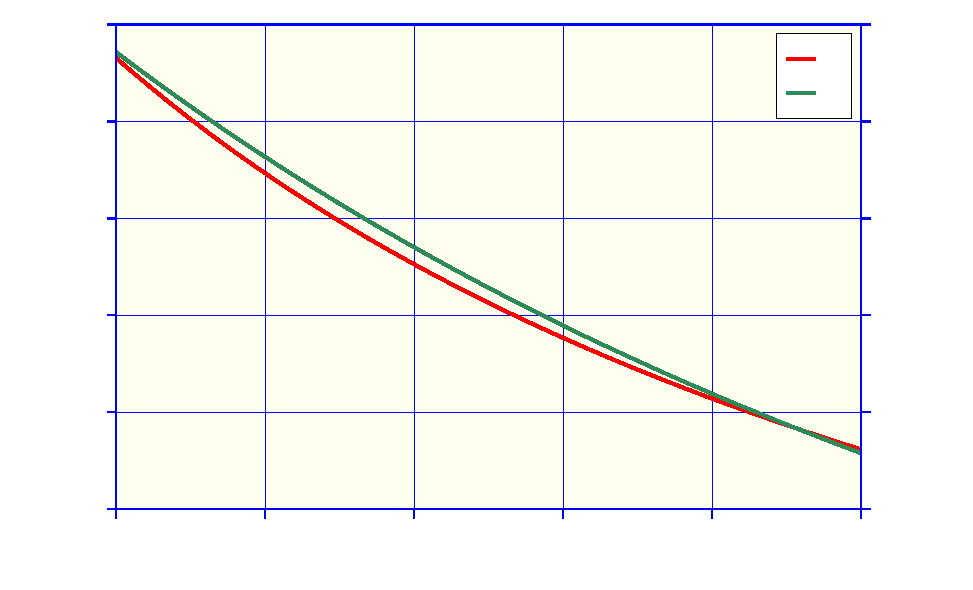
\includegraphics{Cap-Motors-Induccio-Ex8-2-1}}%
    \gplfronttext
  \end{picture}%
\endgroup
